% ex: ts=2 sw=2 sts=2 et filetype=tex
% SPDX-License-Identifier: CC-BY-SA-4.0

\section{Condiciones lógicas y sentencias selectivas}

\begin{frame}[c]{Estructuras selectivas}
  \begin{itemize}
    \item Las \textbf{estructuras selectivas} se utilizan para tomar decisiones
      lógicas y también son conocidas como \textbf{estructuras de decisión} o
      alternativas.
    \pausa
    \item En las estructuras selectivas se evalúa una \textbf{condición} y en
      función del resultado de la misma se realiza una opción u otra.
    \pausa
    \item Las condiciones se especifican usando \textbf{expresiones/condiciones
    lógicas}.
  \end{itemize}
\end{frame}

\begin{frame}[c]{Condiciones lógicas}

  Python admite las condiciones lógicas habituales de las matemáticas:

  \vspace{\baselineskip}
  \begin{itemize}
    \item Es igual a \textbf{a == b}
    \pausa
    \item No es igual a \textbf{a != b}
    \pausa
    \item Menor que \textbf{a < b}
    \pausa
    \item Menor o igual a \textbf{a <= b}
    \pausa
    \item Mayor que \textbf{a > b}
    \pausa
    \item Mayor o igual a \textbf{a >= b}
  \end{itemize}

  \vspace{\baselineskip}
  Estas condiciones se pueden utilizar de varias formas, más
  comúnmente en "sentencias \textcolor{codeKeyword}{if}" y bucles/ciclos.
\end{frame}

\begin{frame}[fragile]
  \frametitle{Sentencias selectivas}

  \begin{columns}
    \column{0.5\textwidth}
    La representación de una estructura selectiva en pseudocódigo.
    \vspace{\baselineskip}
    \begin{lstlisting}[style=pseudocodigo]
Si expresión_lógica Entonces
		acciones_por_verdadero
SiNo
		acciones_por_falso
Fin Si\end{lstlisting}

    \column{0.5\textwidth}
    \pausa
    La representación de una estructura selectiva en diagrama de flujo.
    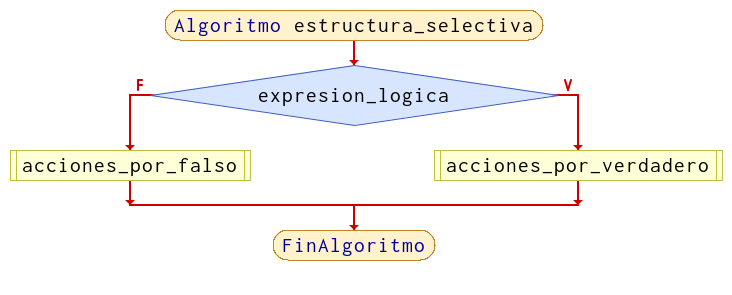
\includegraphics[scale=0.3]{05-sentencia_selectiva.png}
  \end{columns}

  \pausa
  \vspace{\baselineskip}
  La representación de una estructura selectiva en Python.
  \begin{lstlisting}[language=Python]
if expresión_lógica:
		acciones_por_verdadero
else:
		acciones_por_falso
  \end{lstlisting}
\end{frame}

\begin{frame}[fragile]
  \frametitle{Sentencias "si"}

  \begin{columns}
    \column{0.03\textwidth}
    \column{0.6\textwidth}
      Una "instrucción si" se escribe en Python utilizando la palabra clave
      \textcolor{codeKeyword}{if}.

      \vspace{\baselineskip}
      \begin{lstlisting}[language=Python]
  a = 33
  b = 200
  if b > a:
    print("b es más grande que a")\end{lstlisting}

    \column{0.37\textwidth}
    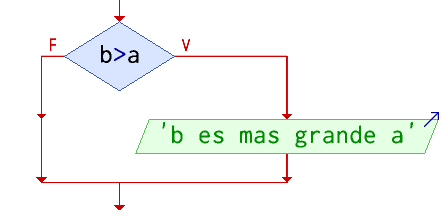
\includegraphics[scale=0.35]{05-if-b-a.png}
  \end{columns}
  En este ejemplo usamos dos variables, a y b, que se usan como parte de
  la instrucción \textcolor{codeKeyword}{if} para probar si b es mayor
  que a. Como a es 33 y b es 200, sabemos que 200 es mayor que 33,
  por lo que imprimimos en la pantalla que "b es mayor que a".
\end{frame}

\begin{frame}[fragile]
  \frametitle{Sangría}

  Python se basa en la \textbf{sangría} (\emph{espacio en blanco al comienzo
  de una línea}) para definir el alcance en el código. Otros lenguajes
  de programación a menudo usan corchetes para este propósito.

  \pausa
  \vspace{\baselineskip}
  \begin{alertblock}{}
    Una sentencia if sin sangría provocará un error.
  \end{alertblock}

  \vspace{\baselineskip}
  \begin{lstlisting}[language=Python]
  a = 33
  b = 200
  if b > a:
  print("b es más grande que a")
  \end{lstlisting}
\end{frame}

\begin{frame}[fragile]
  \frametitle{Elif}

  La palabra clave \textcolor{codeKeyword}{elif} es la forma que usa Python
  para decir "\textbf{si las condiciones anteriores no eran verdaderas,
  entonces pruebe esta condición}".

  \vspace{\baselineskip}
  \begin{lstlisting}[language=Python]
  a = 33
  b = 33
  if b > a:
    print("b es más grande que a")
  elif a == b:
    print("a y b son iguales")
  \end{lstlisting}

  En este ejemplo, a es igual a b, por lo que la primera condición no es
  verdadera, pero la condición \textcolor{codeKeyword}{elif} es verdadera,
  por lo que imprimimos en la pantalla que "\textbf{a y b son iguales}".
\end{frame}

\begin{frame}[fragile]
  \frametitle{Else}

  La palabra clave \textcolor{codeKeyword}{else} captura cualquier cosa que
  no sea detectada por las condiciones anteriores.

  \vspace{\baselineskip}
  \begin{lstlisting}[language=Python]
  a = 200
  b = 33
  if b > a:
    print("b es más grande que a")
  elif a == b:
    print("a y b son iguales")
  else:
    print("a es mayor que b")
  \end{lstlisting}

  En este ejemplo, a es mayor que b, por lo que la primera condición
  \emph{no es verdadera}, también la condición \textcolor{codeKeyword}{elif}
  \emph{no es verdadera}, así que vamos a la condición
  \textcolor{codeKeyword}{else} e imprimimos en la pantalla
  que "\textbf{a es mayor que b}".
\end{frame}

\begin{frame}[fragile]
  \frametitle{if elif else y Pseudocódigo}

  Para escoger un valor entre varios se usa:
  \begin{columns}
    \column{0.02\textwidth}
    \column{0.525\textwidth}
      \begin{lstlisting}[language=Python]
num = eval(input("Escribe un número: "))
if num == 1:
  print("Escogiste 1")
elif num == 2:
  print("Escogiste 2")
elif num == 3:
  print("Escogiste 3")
elif num == 4:
  print("Escogiste 4")
else:
  print("Escogiste otro número")
      \end{lstlisting}
    \pausa
    \column{0.49\textwidth}
      \begin{lstlisting}[style=pseudocodigo]
Escribir "Escribe un número:"
Leer num
Segun num Hacer
  1:
    Escribir "Escogiste 1"
  2:
    Escribir "Escogiste 2"
  3:
    Escribir "Escogiste 3"
  4:
    Escribir "Escogiste 4"
  De Otro Modo:
    Escribir "Escogiste otro número"
Fin Segun
      \end{lstlisting}
  \end{columns}
\end{frame}

\begin{frame}[fragile]
  \frametitle{Else}

  Se puede tener \textcolor{codeKeyword}{else} sin el
  \textcolor{codeKeyword}{elif}

  \begin{columns}
    \column{0.02\textwidth}
    \column{0.50\textwidth}
      \begin{lstlisting}[language=Python]
  a = 200
  b = 33
  if b > a:
    print("b es más grande que a")
  else:
    print("b NO es mayor que a")
      \end{lstlisting}
    \pausa
    \column{0.02\textwidth}
    \column{0.49\textwidth}
      \begin{lstlisting}[style=pseudocodigo]
  a <- 200
  b <- 33
  Si b > a Entonces
    Escribir "b es más grande que a"
  SiNo
    Escribir "b NO es mayor que a"
  Fin Si
      \end{lstlisting}
  \end{columns}
\end{frame}

\begin{frame}[fragile]
  \frametitle{Manera corta del if}

  Si solo tiene una instrucción para ejecutar, puede ponerla en la misma
  línea que la instrucción if.

  \vspace{\baselineskip}
  \begin{lstlisting}[language=Python]
  if a > b: print("a es mayor que b")
  \end{lstlisting}
\end{frame}

\begin{frame}[fragile]
  \frametitle{Manera corta del if ... else}

  Si solo tiene una declaración para ejecutar, una para if y otra para
  else, puede ponerlas todas en la misma línea:

  \vspace{\baselineskip}
  \begin{lstlisting}[language=Python]
  a = 2
  b = 330
  print("A") if a > b else print("B")
  \end{lstlisting}

  \vspace{\baselineskip}
  \begin{exampleblock}{}
    Esta técnica se conoce como \textbf{operadores ternarios} o
    \textbf{expresiones condicionales}.
  \end{exampleblock}
\end{frame}

\begin{frame}[fragile]
  \frametitle{Manera corta del if ... else}

  También puede tener varias declaraciones else en la misma línea:

  \vspace{\baselineskip}
  \begin{lstlisting}[language=Python]
  a = 2
  b = 330
  print("A") if a > b else print("=") if a == b else print("B")
  \end{lstlisting}

  \vspace{\baselineskip}
  \begin{block}{Lo podemos leer como:}
    Imprime A si a es mayor que b si no, imprime = si a es igual a b, y si
    no, imprime B
  \end{block}
\end{frame}

\begin{frame}[fragile]
  \frametitle{And}

  La palabra clave \textcolor{codeKeyword}{and} es un operador lógico y
  se utiliza para combinar declaraciones condicionales:

  \vspace{\baselineskip}
  \begin{lstlisting}[language=Python]
  a = 200
  b = 33
  c = 500
  if a > b and c > a:
    print("Ambas condiciones son verdaderas")
  \end{lstlisting}
\end{frame}

\begin{frame}[fragile]
  \frametitle{Or}

  La palabra clave \textcolor{codeKeyword}{or} es un operador lógico y
  se utiliza para combinar declaraciones condicionales:

  \vspace{\baselineskip}
  \begin{lstlisting}[language=Python]
  a = 200
  b = 33
  c = 500
  if a > b or a > a:
    print("Al menos una condicion es verdaderas")
  \end{lstlisting}
\end{frame}

\begin{frame}[fragile]
  \frametitle{If anidados}

  Puede tener sentencias if dentro de sentencias if, esto se llama
  \textbf{sentencias if anidadas}.

  \begin{columns}
    \column{0.55\textwidth}
    \begin{lstlisting}[style=pseudocodigo]
Si x > 10 Entonces
  Escribir "mayor que diez,"
  Si x > 20 Entonces
    Escribir "y también mayor que 20!"
  SiNo
    Escribir "pero menor que 20."
  Fin Si
Fin Si\end{lstlisting}
    \column{0.45\textwidth}
    \pausa
    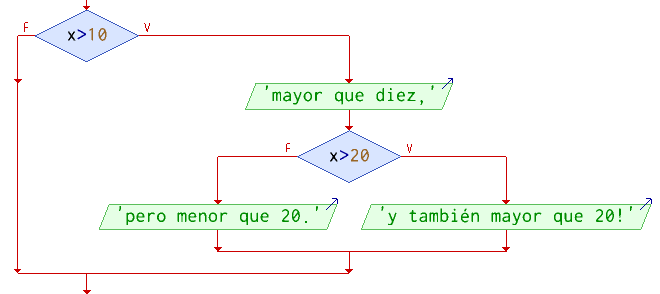
\includegraphics[scale=0.3]{05-if-x-10-if-x-20.png}
  \end{columns}
\end{frame}

\begin{frame}[fragile]
  \frametitle{If anidados}

  El código en Python sería:

  \vspace{\baselineskip}
  \begin{lstlisting}[language=Python]
  x = 41

  if x > 10:
    print("mayor que diez,")
    if x > 20:
      print("y tambien mayor que 20!")
    else:
      print("pero menor que 20.")
  \end{lstlisting}
\end{frame}

\begin{frame}[fragile]
  \frametitle{La sentencia \textbf{pass}}

  Las declaraciones if no pueden estar vacías, pero si por alguna razón
  tiene una declaración if sin contenido, coloque la declaración pass
  para evitar errores.

  \vspace{\baselineskip}
  \begin{lstlisting}[language=Python]
  a = 33
  b = 200

  if b > a:
    pass
  \end{lstlisting}
\end{frame}

